\section{Model baze podataka sistema}
\indent
\indent
\begin{figure}[H]
\makebox[\textwidth][c]{%
    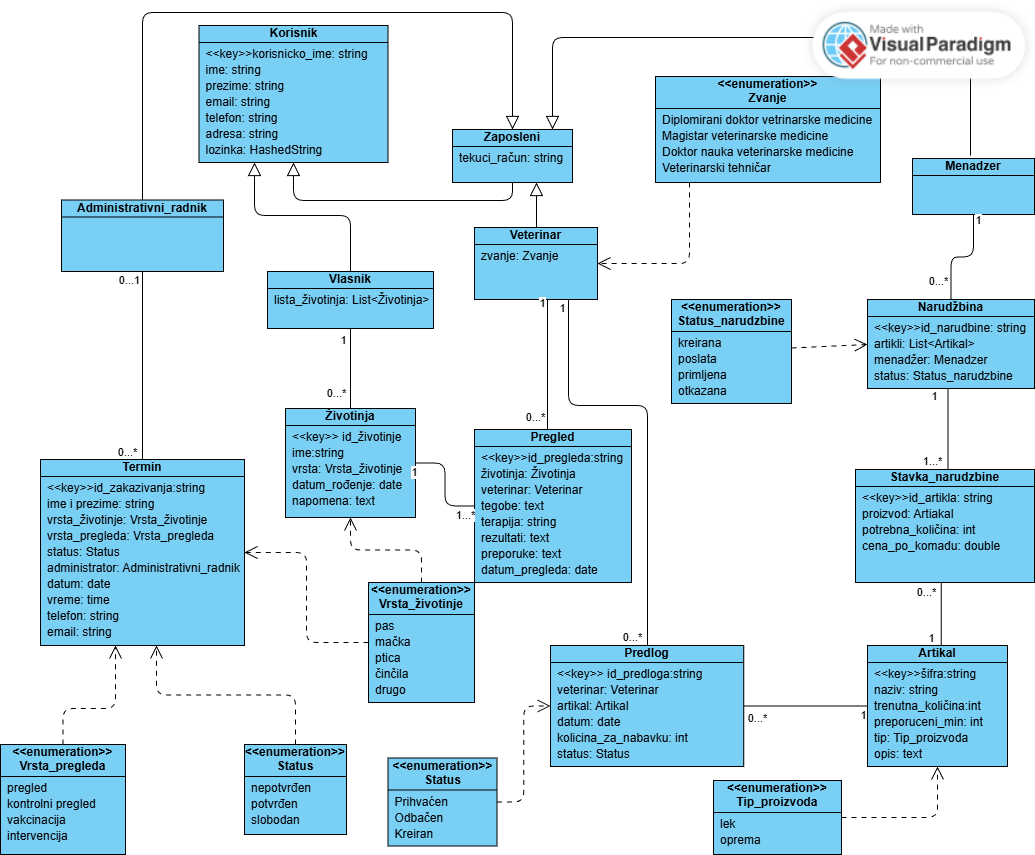
\includegraphics[width=1.3\textwidth]{Dijagrami/dijagram_klasa.png}
}
\caption{Dijagram klasa podataka}
\label{fig:dijagram-klasa}
\end{figure}
\newpage
\subsection{Opis modela}
\indent U ovom modelu baze podataka ključni entiteti su vlasnik, životinja, termin pregleda, karton životinje, pregled, tretman, kao i entiteti vezani za upravljanje zalihama lekova i medicinske opreme. Entitet vlasnik je povezan sa jednom ili više životinja, dok svaka životinja ima svoj karton u okviru kog se čuvaju podaci o pregledima, dijagnozama i tretmanima. Entitet termin omogućava evidenciju zakazivanja, izmene i otkazivanja pregleda. Pored medicinskog dela sistema, model obuhvata i entitete artikal, potrošnja i narudžbenica, koji omogućavaju praćenje stanja zaliha, evidenciju potrošnje i blagovremenu nabavku lekova i opreme. Na ovaj način model baze podataka podržava osnovne poslovne procese veterinarske klinike.
\subsection{Entiteti i veze}

\indent\textbf {Korisnik}
\begin{itemize}
    \item Opis: Klasa korisnik predstavlja najapstraktniji opis korisnika i povezana je sa tabelom u bazi.
    \item Atributi: ime, prezime, email, broj\_telefona, adresa, lozinka
\end{itemize}

\indent\textbf {Vlasnik}
\begin{itemize}
    \item Opis: Izvedena klasa klase Korisnik
    \item Jedan vlasnik može imati 0 ili vise Životinja (0:N)
\end{itemize}

\indent \textbf{Zaposleni}
\begin{itemize}
    \item Opis: Izvedena klasa klase Korisnik, predstavlja apstrakciju svih korisnika koji su zaposleni na klinici
    \item Atributi: broj računa
\end{itemize}

\indent \textbf{Veterinar}
\begin{itemize}
    \item Opis: Izvedena klasa klase Zaposleni
    \item Atributi: zvanje
    \item Jedan veterinar može imati 0 ili vise Pregled (0:N)
    \item Jedan veterinar može imati 0 ili vise Predloga (0:N)
\end{itemize}

\indent \textbf{Administrativni radnik}
\begin{itemize}
    \item Opis: Izvedena klasa klase Zaposlenis
    \item Jedan Administrativni radnik može imati 0 ili više Termina (0:N)
\end{itemize}

\indent \textbf{Menadzer}
\begin{itemize}
    \item Opis: Izvedena klasa klase Zaposleni 
    \item Jedan Administrativni radnik može imati 0 ili više Narudzbina (0:N)
\end{itemize}

\indent\textbf{Životinja}
\begin{itemize}
    \item Opis: Klasa kojoj odgovara tabela koja sadrži osnovne podatke o ljubimcu koji se leči u veterinarskoj klinici.
    \item Atributi: id životinje (broj kartona), ime, vrsta, datum rođenja, vlasnik (FK u tabeli)
    \item Životinj jednog Vlasnika (1)
    \item Životinja može imati 0 ili više Pregleda (0:N)
\end{itemize}

\indent\textbf{Pregled}
\begin{itemize}
    \item Opis: Klasa kojoj odgovara tabela koja sadrži podatke o pojedinačnim pregledima životinje koje obavlja veterinar.
    \item Atributi: id pregleda, životinja (FK u tabeli), vetarinar (FK u tabeli), datum, tegobe, terapija, rezultati, preporuke
    \item Pregled obavlja jedan veterinar (1)
    \item Pregled obavlja jedan nad jednom Životinjom (1)
\end{itemize}

\indent\textbf{Predlog}
\begin{itemize}
    \item Opis: Klasa kojoj odgovara tabela koja sadrži podatke o predlozima veterinara o nabavci opreme.
    \item Atributi: id veterinar (FK u tabeli), artikal (FK u tabeli), datum, količina, status
    \item Jedan predlog kreira jedan veterinar (1)
\end{itemize}

\indent\textbf{Termin}
\begin{itemize}
    \item Opis: Klasa kojoj odgovara tabela koja sadrži termine za naredna 3 meseca.
    \item Atributi: id termina, ime, vrsta životinje, vrsta pregleda, status, administrativni radnik (FK u tabeli), datume, vreme, telefon, email
    \item Jedan administrativni radnik menja 0 ili više termina (0:N)
\end{itemize}

\indent\textbf{Artikal}
\begin{itemize}
    \item Opis: Klasa kojoj odgovara tabela koja sadrži podatke o lekovima ili medicinskoj opremi dostupnoj u klinici.
    \item Atributi: id, naziv, količina, preporučena količina, tip, opis
    \item Jedan artikal je sadržan u 0 ili više Predloga (0:N)
    \item Jedan artikal je sadržan u u 0 ili više Stavki Narudžbine (0:N)
\end{itemize}

\indent\textbf{Stavka narudžbine}
\begin{itemize}
    \item Opis: Klasa kojoj odgovara tabela koja sadrži podatke o količini i ceni pojedinačnih artikala koje treba nabaviti
    \item Atributi: id, artikal (FK u tabeli), narudžbina (FK u tabeli)
    \item Stavka odgovara tačno jednoj narudžbini (1)
    \item Stavka odgovara tačno jednom Artiklu (1)
\end{itemize}

\indent\textbf{Narudžbina} - podaci o naručivanju lekova i opreme.
\begin{itemize}
    \item Opis: Klasa kojoj odgovara tabela koja sadrži podatke jednoj narudžbini
    \item Atributi: id, menadžer (FK u tabeli), status
    \item Narudžbina može imati 0 ili više stavki (0:N)
    \item Svakom naruđbinom upravlja jedan menadžer (1)
\end{itemize}













